\section{Détail de la conception de la partie microcontrôleur du projet}
	\subsection{Le capteur}
		Lors de la réalisation du senseur il a fallu en premier lieu se fixer
		des objectifs à atteindre, afin d'être sûr d'aller dans une direction
		cohérente tout au long du projet. De  ce fait nous avons choisi d'opter pour
		la réalisation d'un prototype fonctionnel et relativement simple au début.
		Par relativement simple, nous entendions capable de lire un ou deux capteurs
		analogiques simples à mettre en place de manière à nous focaliser sur
		l'interfaçage du dispositif avec un serveur de données. Nous nous sommes
		donc d'avantage focalisés sur une approche plus logicielle du projet en
		écartant volontairement, par manque de temps, des considérations annexes
		comme la gestion de l'énergie ou la mise en place immédiate de capteurs
		très complexes. Le but était réellement de fournir une base saine sur laquelle
		il serait facile de s'appuyer à l'avenir.
		
		\subsubsection{La partie électronique}
		
		La partie électronique est la plus simple de l'appareil c'est donc celle
		là qui sera abordée en premier. Elle se compose simplement d'une photo résistance
		montée en pull up sur la patte analogique 1 de l'Arduino et d'un capteur de
		température câblé sur la patte analogique 2. Nous avons également câblé un bouton de
		mise à jour (dont l'utilité sera détaillée plus tard) sur la patte PD2
		ainsi que la real time clock sur trois pattes numériques de manière à pouvoir
		échanger des données. Tout ces composants ont été positionnés sur une breadboard
		de manière à ce que nous puissions facilement en modifier l'arrangement au fur et a mesure
		que nos besoins évoluaient dans le projet.
		\par
		Nous n'avons malheureusement pas eu le temps de réaliser de carte
		pour fixer ce design. Et il n'aurait pas été pertinent de le faire dans la mesure
		ou la conception, le routage et la fabrication d'une carte sont des activités pour
		le moins chronophages et qu'il a effectivement été plus productif pour nous de nous
		concentrer sur l'ajout de nouvelles fonctionalités au capteur. Cependant
		nous avons édités des PCB et des schémas électroniques disponibles en
		annexe qui permettent de réaliser une telle carte.
		
		\subsubsection{Conception du firmware de l'Arduino}
		La conception du firmware de l'arduino s'est découpée en plusieurs étapes.
		Pour commencer nous avons séparé les différentes fonctionnalités que nous
		souhaitions. D'un point de vue organisation cela s'est traduit par un fractionnement
		du code en plusieurs fichiers, chacun regroupant les fonctions relatives à un
		domaine, par exemple la gestion du port série, des CAN, de l'EEPROM et autre.
		\par
		Ensuite, une fois que la séparation logique des fonctionalités a été effectuée
		nous avons commencé à les développer une à une, en lançant à chaque fois une
		série de tests sur ce que nous avions créé, de manière à nous assurer que tout
		était bien conforme à ce que nous attendions. De cette manière nous pouvions
		réutiliser sans crainte le code que nous avions précédemment écrit puisqu'il
		avait été validé par une batterie de tests.
		\par
		Une attention toute particulière a été portée à la documentation. En effet si nous
		souhaitons que le projet puisse être repris les années suivantes il
		est indispensable de fournir une documentation valable, fiable et complète
		de manière à ce que n'importe qui ou presque soit en mesure de comprendre
		ce qui a déjà été réalisé de manière logicielle. Pour ce faire nous avont eu
		recours au système de documentation in-code Doxygen, qui grâce à un
		système de commentaires au formattage particulier permet de générer automatiquement
		une belle documentation HTML. Cette documentation navigable est facile à utiliser, avec outils
		de recherche intégré et liens entre les différentes fonctions documentées.
		Si vous souhaitez construire la documentation du programme rendez vous dans
		le répertoire Arduino et tapez simplement \texttt{doxygen} un dossier contenant
		le nécessaire sera généré pour vous !
		\par
		La seconde partie du projet, qui n'est au final même pas utilisée dans le prototype
		actuel, a été la réalisation d'un driver pour la real time clock de Maxim DS1302.
		Ce driver a été implémenté en utilisant le protocole de communication 3-Wire décrit dans
		la datasheet, c'est un protocole similaire au protocole SPI mais suffisamment différent de celui ci
		pour ne pas pouvoir utiliser le contrôleur SPI de l'Arduino. Le driver est fonctionnel et
		permet d'accéder aux registres de temps de la RTC ainsi qu'aux quelques octets de RAM qu'elle
		nous fourni en plus, ce qui peut être pratique si jamais l'arduino venait à en manquer. Toutes
		les informations nécessaires sont bien évidemment documentées dans le code et via Doxygen.
		\par
		Nous somme partis du constat que le fonctionnement du WiFi pouvait être parfois
		assez instable, et que de ce fait il serait appréciable que le capteur puisse se comporter
		comme une sorte de datalogger dans le cas où il serait dans l'incapacité momentanée de communiquer
		avec le serveur de donnée, que cela soit a cause du wifi ou d'un autre problème d'ailleurs.
		Pour cela nous avions pensé le coupler avec une flash (voir les schémas en annexe). Cela dit
		comme le composant n'était disponible qu'en format SOIC8 et que nous n'avons pas réalisé la carte
		il nous a été impossible de l'intégrer correctement. Une amélioration possible et très facile à
		mettre en oeuvre pour le projet serait donc l'intégration de cette flash et l'utilisation
		de la RTC pour soumettre en différé des données de mesures qui n'auraient pas pu être
		transmises à temps.
		\par
		La troisième partie du projet a été consacrée à faire en sorte que la configuration du capteur
		soit persistante entre les reboots. Durant les phases de développement nous ne nous étions pas
		vraiment occupés de cela mais dès que le programme est devenu plus compliqué il est devenu
		essentiel de stocker certains paramètres (d'identifications notamment) autrement qu'en dur
		dans le code. Il a donc fallu ajouter un module de gestion de l'EEPROM. La structure suivante a donc
		été choisie pour stocker des données :
		\begin{itemize}
			\item L'EEPROM est découpée en différents secteur de taille fixé à la compilation
			\item Chaque secteur contient un octet de taille et $N$ octets de données ($N < 255$)
			\item Chaque secteur est uniquement défini par sa position en mémoire
		\end{itemize}
		
		Cette solution présente l'avantage d'être très simple à mettre en place d'un point de vue
		logiciel, ce système souffre cependant d'un gros problème qui est que l'on ne peut
		pas connaître de manière dynamique la taille maximale des données que l'on peut ranger
		dans un segment. Ce qui implique que le programmeur fasse très attention aux données qu'il
		manipule, de manière à ne pas provoquer de débordement sur un autre segment. Ceci dit,
		ce problème n'est pas vraiment critique puisqu'une simple réécriture de la configuration
		rétablira tout correctement. Ceci fait également partie des améliorations possibles
		du projet.
		
		\par
		La quatrième partie du projet a sans aucun doute été la plus difficile à réaliser. En
		effet après s'être occupé des briques élémentaire qui compose le capteur (communiquer
		en série, lire des capteurs analogiques, lire la RTC). Il a fallu regrouper tout ça
		ensemble et l'envoyer sur internet. Pour se faire, il a d'abord fallu comprendre comment
		fonctionnait la carte WiFi. La datasheet n'étant pas toujours très claire, ni très complète
		il a d'abord fallu passer par une phase \og{} d'exploration \fg{} de la carte via le port
		série, de manière à comprendre précisément ce qu'elle attendait de nous en terme de commandes.
		La carte se configurait finalement par un set de commandes AT via le port série et malgré
		les quelques imprécisions de la datasheet nous avons finalement été capables de nous identifier
		sur un réseau spécialement créé pour l'occasion.
		
		\par
		A partir de là a été développé une petite bibliothèque qui intègre les fonctions réseau de base,
		à savoir s'identifier sur un réseau avec des paramètres donnés, soumettre des requêtes HTTP et
		vérifier le retour des commandes AT de manière à réitérer plusieurs fois une tentative de connexion
		qui aurait échoué. Cette bibliothèque fonctionne sur le port série via une scrutation, elle n'utilise
		pas d'interruptions pour avoir plus de contrôle et intercepter tout ce qui circule sur le port série
		et le conserver au sein du même contexte (il est préférable que le retour d'une commande reste interceptée
		par la fonction qui l'a émise plutôt que de devoir passer par une interruption globale et deviner
		quelle fonction a besoin des données reçues).
		
		\subsubsection{Communication avec l'application web}
		Une fois la carte configurée et connectée au réseau, il a fallu envoyer des données de mise à jour au
		site de Benoit. Nous avions au départ pensé à faire ça via post en JSON, simplement ça aurait
		été trop long et gourmand à mettre en place niveau mémoire (les données post doivent avoir
		une longueur définie et il faut encoder les caractères "{:," qui sont très utilisées dans une
		chaine JSON ce qui aurait rendu l'envoi des données affreuse). Du coup nous avons opté pour un
		format d'envoi en post classique. Voici par exemple la requête POST que le capteur "cap1" doté du mot de passe
		"coucoutuveuxvoirmadata" aurait envoyé :
		
		\begin{verbatim}
    POST /recup.php HTTP/1.0
    Host: smartsensorwifi.plil.net
    Content-type: application/x-www-form-urlencoded
    Content-length: 100
    
    temp=140&lum=17&mid=cap1&mpass=coucoutuveuxvoirmadata
		\end{verbatim}
		
		\par Notons que les valeurs envoyées peuvent paraître étranges, mais elle ne sont que la lecture
		directe du CAN de l'ATmega, la serveur les traitera pour les transformer en température ou
		déterminer le seuil de luminosité. Ainsi on décharge le microcontrôleur d'une partie
		du travail.
		
		\subsubsection{Reconfiguration du capteur}
		Une fois que le projet est capable de communiquer avec l'appli web, de soumettre
		des données, de se connecter à un réseau et ce genre de chose il ne lui manque pas beaucoup de fonctionnalités.
		Ceci dit une fonctionnalité indispensable s'est vite faite ressentir :
		le besoin de pouvoir reconfigurer le capteur à distance. En effet, le
		seul moyen de reconfigurer le capteur était en modifiant en dur dans le code les identifiants et
		de reflasher le programme ensuite, ce qui n'est pas pratique.

		Pour palier à ce problème nous avons donc créé un set relativement complet de commandes AT,
		documentées en annexe. L'idée est que le capteur écoute ce qu'il se passe sur son port série
		et dès qu'une commande AT est reconnue elle est exécutée pour peu que l'on soit authentifié sur
		le capteur. Pour se faire nous avons établi deux modes de configuration, une configuration "locale" via
		le port série, et une reconfiguration à distance via le réseau. 
		
		\subsubsection{Principales difficultés rencontrées}
		
	\subsection{Configurator.py}
	\begin{wrapfigure}{r}{40mm}
		  \centering
		  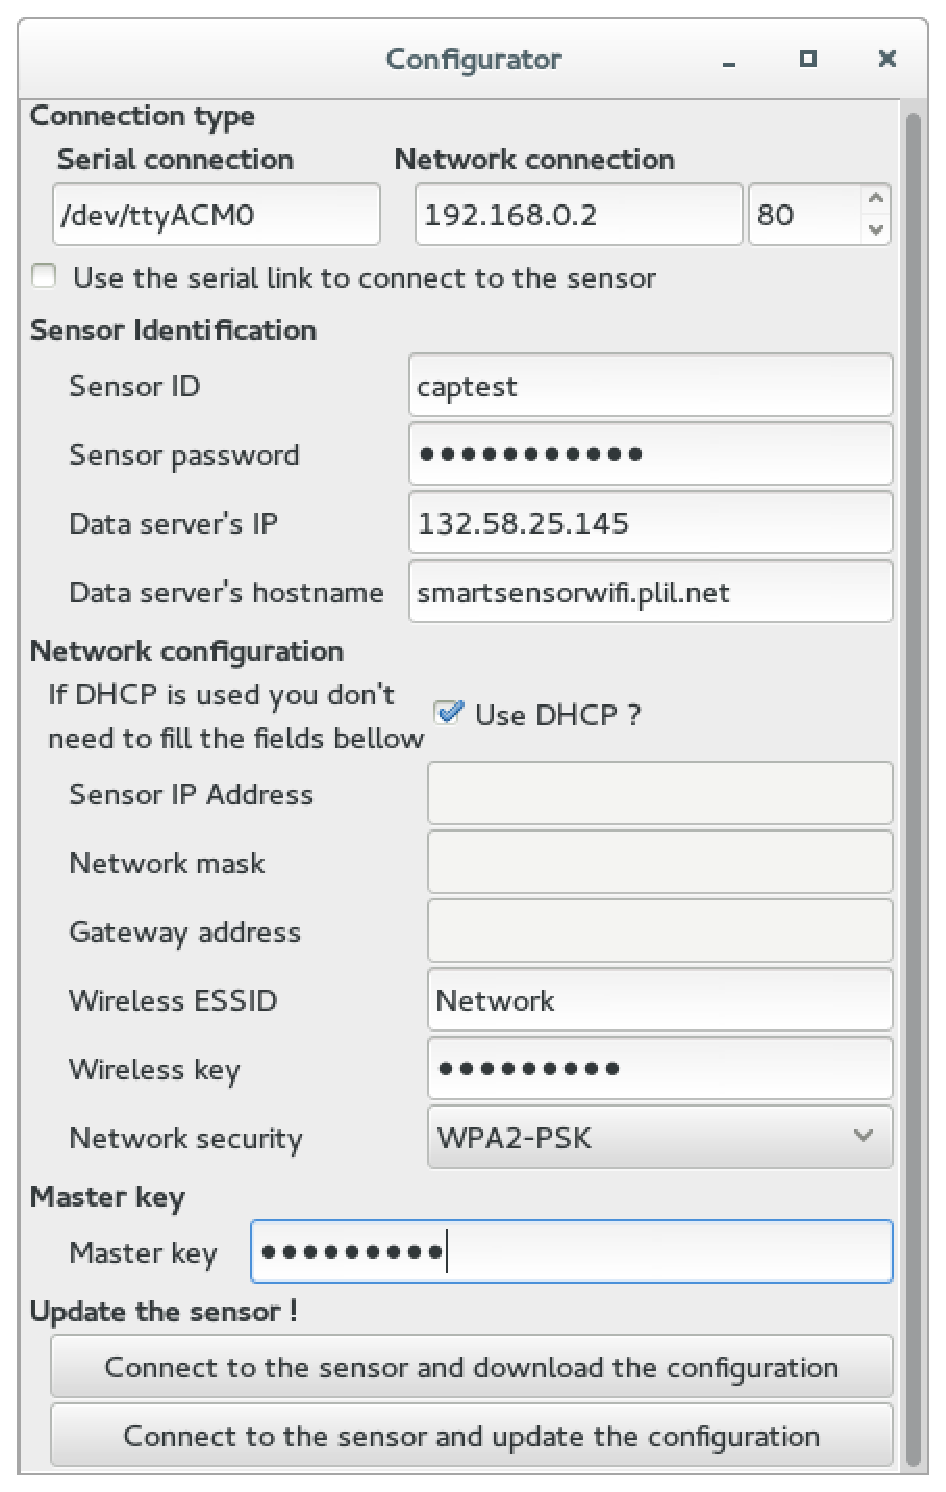
\includegraphics[scale=0.3]{SSWconfigurator.eps}
		  \caption{Interface de configurator}
		  \vspace{-20mm}
	\end{wrapfigure}
		Afin que l'utilisateur n'ai pas a se munir de minicom ou de netcat pour reconfigurer
		ses capteurs, nous avons choisi de développer un logiciel dont le rôle est de se
		charger de la configuration à la place de l'utilisateur. Qu'il s'agisse d'une configuration
		locale via le port série ou à distance via le réseau, configurator fait le lien
		entre l'utilisateur et son capteur. Le logiciel dispose d'une interface très simple composée
		de quelques champs et de deux boutons, un pour rapatrier la configuration d'un capteur et l'autre
		pour envoyer une configuration à un capteur. De cette manière il n'est plus utile de connaître
		par coeur les commandes AT nécessaires à la configuration de l'appareil. Ce logiciel a été
		réalisé en python avec pygtk, glade2 et pyserial.
	
	\subsection{Tentative de substitution par une solution a base de RaspberryPi}
		Comme la carte WizFi tardait à arriver, nous avons pensé opter pour une solution alternative
		pour réaliser le capteur, à base d'une RaspberryPi. Certes la solution était un peu surdimensionnée
		pour ce que l'on voulait en faire, mais comme cela on aurait eu quelque chose de fonctionnel
		à montrer lors de la soutenance. L'idée était d'utiliser les GPIO de la Raspberry pour
		l'interfacer avec le monde exterieur.
		\par
		Malheureusement la RaspberryPi est un appareil qui ne dispose pas d'entrées analogiques,
		ce qui est assez peu pratique pour lire une température ou une luminosité de la même manière que
		sur un ATmega. Nous avons donc dû recourir à un ADC externe fonctionnant suivant le protocole SPI,
		ce qui tombait plutôt bien puisque la Raspberry est équipée d'une inetrface SPI lui permettant
		de contrôler jusqu'à deux esclaves. Pour notre problème nous avons opté pour l'ADC MCP3208 de
		MicroChip. Pourquoi celui là ? Tout simplement parce qu'il dispose de huit canaux analogiques ce qui
		permet une grande variété de capteurs, mais également parce qu'il peut fonctionner en 3v3, tension à
		laquelle fonctionne également la Raspberry, ainsi on évite de la griller.
		\par
		J'ai donc réalisé une carte et un PCB pour réaliser cette alternative, mais également
		la couche logicielle qui va avec. J'ai en effet développé une classe en C++ qui
		encapsule tout les appels systèmes permettant d'écrire et de lire sur le port SPI
		de la raspberry, en full duplex. J'ai en réalité réalisé deux classes, une classe
		SPI qui est la classe mère, comprenant seulement les routines d'initialisation et d'écriture
		du port SPI, et une SPI\_MCP3208 qui comprend les commandes spécifiées dans la datasheet
		du composant.
		\par
		Pour information, cette classe et le programme d'exemples sont disponibles sur GitHub et la
		documentation est disponible à l'addresse spécifiée dans le wiki du projet.
		\par
		Cela dit, il y a eu un problème, il était que les données renvoyées par l'ADC étaient
		totalement incohérentes. Le fait est qu'à luminosité égale, si on lançait 10 acquisitions
		nous pouvions obtenir des écarts de plus de 3000 (sur 4095 d'amplitude) entre
		deux valeurs, quand bien même la luminosité ne variait pas. Le plus déroutant
		dans tout cela c'est que le problème n'avait pas l'air de venir de notre logiciel,
		dans la mesure ou nous étions parfaitement capables, avec la même couche logicielle,
		de piloter d'autre appareils SPI fonctionnant en esclave (comme un afficheur 4x7
		segments de chez SparkFun par exemple). La seconde chose la plus dérourante était
		que les données étaient cohérentes du point de vue du fonctionnement du composant
		tel que décrit dans la datasheet. Je m'explique, une trame classique de communication avec
		l'ADC se compose comme il suit (schématiquement) :
		\\
		\texttt{4 bits de commande | deux bits de sample | 12 bits de résultat MSB first}\\

		Le fait est que d'après la datasheet en continuant à envoyer des coups d'horloge
		au composant après le dernier bit de donnée, le composant va nous renvoyer le
		résultat de la conversion mais LSB first. On récupère donc le symétrique des données
		par rapport au LSB. Après avoir analysé plusieurs séquences nous avons pu constater que
		l'erreur ne venait pas de la manière dont nous récupérions nos données puisqu'elles étaient
		correctes du point de vue de la datasheet mais totalement aberrantes d'un point de vue physique.
		\par
		L'erreur ne venait pas non plus du hardware puisqu'un rapide coup d'oeil à l'oscilloscope nous a
		permis de constater que la tension sur la patte de l'ADC évoluait bien comme elle le devait.
		Le mystère est resté entier puisqu'après nous avons reçu la carte WizFi et nous avons pu commencer
		à travailler dessus, cette solution a donc été abandonnée. Cela dit, nous avions déjà commencé à
		réfléchir aux technologies que nous aurions pu mettre en place pour réaliser la solution, qui auraient été :
		\begin{itemize}
			\item Un programme de lecture des données appelé par cron à intervalle régulier (un bête script bash
			qui lit le port SPI et conditionne les données en POST par exemple pour les envoyer au site de Benoît)
			\item Une application Web similaire à celle de Benoît mais ne concernant que les données locales
			de l'appareil, qui aurait permis de modifier les paramètres de mises à jour/sécurité tout
			simplement depuis un navigateur. Nous avions pensés à la réaliser en Python avec CherryPy un
			excellent framework python très léger, et évidemment Ink pour le design. 
		\end{itemize}
